\subsection{构造检验的方法}\label{sec:8.2}
我们将详细讨论四种构造检验程序的方法，它们适用于不同情形，利用问题的不同方面. 首先介绍一种非常一般的方法，它几乎总能应用，而且在某些情况下还是最优的.
\subsubsection{似然比检验}\label{sec:8.2.1}
假设检验的似然比方法与\autoref{sec:7.2.2}讨论的最大似然估计量有关，似然比检验的适用范围也与最大似然估计一样广泛. 回顾，若 $X_1,\ldots,X_n$ 是来自密度或质量函数为 $f(x\mid\theta)$ 的总体的随机样本（$\theta$ 可以是向量），则似然函数定义为
$$L(\theta\mid x_1,\ldots,x_n)=L(\theta\mid\boldsymbol x)=f(\boldsymbol x\mid\theta)=\prod_{i=1}^n f(x_i\mid\theta).$$
用 $\Theta$ 表示整个参数空间. 似然比检验定义如下.
\begin{definition}\label{def:8.2.1}\index{SI0630@似然比检验}
检验 $H_0:\theta\in\Theta_0$ 对 $H_1:\theta\in\Theta_0^c$ 的似然比检验统计量（likelihood ratio test statistic）为
$$\lambda(\boldsymbol x)=\frac{\sup_{\Theta_0}L(\theta\mid\boldsymbol x)}{\sup_\Theta L(\theta\mid\boldsymbol x)}.$$
似然比检验（likelihood ratio test，LRT）是拒绝域形如 $\{\boldsymbol x:\lambda(\boldsymbol x)\le c\}$ 的任一检验，其中 $c$ 是满足 $0\le c\le1$ 的任意数.
\end{definition}
当 $f(\boldsymbol x\mid\theta)$ 是离散随机变量的概率质量函数时，或许最容易理解似然比检验背后的道理. 此时，$\lambda(\boldsymbol x)$ 的分子是已观察样本的最大概率，最大值在原假设中的参数上计算（见\autoref{exercise:8.4}\mbox{）.} 分母则是已观察样本在所有可能参数上的最大概率. 若备择假设中存在某些参数点，使已观察样本比在原假设任一参数点下都可能得多，那么这两个最大值之比就很小. 此时，似然比检验准则认为应当拒绝 $H_0$，接受 $H_1$ 为真. 选择数值 $c$ 的方法将在\autoref{sec:8.3}讨论.

\sourcepageanchor{335}
如果把最大化区分为在整个参数空间上进行的无约束最大化（unrestricted maximization），以及在参数空间子集上进行的约束最大化（restricted maximization），似然比检验与最大似然估计量的联系就更清楚了. 假设 $\theta$ 的一个最大似然估计量 $\hat\theta$ 存在，它由对 $L(\theta\mid\boldsymbol x)$ 作无约束最大化得到. 也可以把 $\Theta_0$ 看作参数空间，考虑约束最大化所得的 $\theta$ 的最大似然估计量，记为 $\hat\theta_0$.\index{SI0635@最大似然估计量}\semanticindexanchor{635:335}\index{SI0678@似然比检验}\semanticindexanchor{678:335} 即 $\hat\theta_0=\hat\theta_0(\boldsymbol x)$ 是使 $L(\theta\mid\boldsymbol x)$ 最大的 $\theta\in\Theta_0$ 的值. 于是似然比检验统计量为
$$\lambda(\boldsymbol x)=\frac{L(\hat\theta_0\mid\boldsymbol x)}{L(\hat\theta\mid\boldsymbol x)}.$$
\begin{example}[正态总体的似然比检验]\label{ex:8.2.2}\index{SI0638@正态}
设 $X_1,\ldots,X_n$ 是来自 $\mathrm n(\theta,1)$ 总体的随机样本. 考虑检验 $H_0:\theta=\theta_0$ 对 $H_1:\theta\ne\theta_0$，其中 $\theta_0$ 是实验者在实验前固定的数. 由于 $H_0$ 只规定一个 $\theta$ 值，$\lambda(\boldsymbol x)$ 的分子为 $L(\theta_0\mid\boldsymbol x)$. \autoref{ex:7.2.5}已求出 $\theta$ 的无约束最大似然估计量是样本均值 $\bar X$，所以分母为 $L(\bar x\mid\boldsymbol x)$. 因此，似然比检验统计量为
\begin{equation}\label{eq:8.2.1}
\begin{aligned}
\lambda(\boldsymbol x)&=\frac{(2\pi)^{-n/2}\exp[-\sum_{i=1}^n(x_i-\theta_0)^2/2]}{(2\pi)^{-n/2}\exp[-\sum_{i=1}^n(x_i-\bar x)^2/2]}\\
&=\exp\left[\left(-\sum_{i=1}^n(x_i-\theta_0)^2+\sum_{i=1}^n(x_i-\bar x)^2\right)/2\right].
\end{aligned}
\end{equation}
注意到
$$\sum_{i=1}^n(x_i-\theta_0)^2=\sum_{i=1}^n(x_i-\bar x)^2+n(\bar x-\theta_0)^2,$$
就可化简 $\lambda(\boldsymbol x)$，得到
\begin{equation}\label{eq:8.2.2}
\lambda(\boldsymbol x)=\exp[-n(\bar x-\theta_0)^2/2].
\end{equation}
似然比检验在 $\lambda(\boldsymbol x)$ 较小时拒绝 $H_0$. 由\eqref{eq:8.2.2}，拒绝域 $\{\boldsymbol x:\lambda(\boldsymbol x)\le c\}$ 可写为
$$\{\boldsymbol x:|\bar x-\theta_0|\ge\sqrt{-2(\log c)/n}\}.$$
当 $c$ 在 $0$ 与 $1$ 之间变化时，$\sqrt{-2(\log c)/n}$ 在 $0$ 与 $\infty$ 之间变化. 因而，似然比检验就是当样本均值与假设值 $\theta_0$ 的差超过某个指定量时，拒绝 $H_0:\theta=\theta_0$ 的那些检验.
\end{example}
\autoref{ex:8.2.2}中的分析是典型的：先按\autoref{def:8.2.1}求出 $\lambda(\boldsymbol X)$ 的表达式，如\eqref{eq:8.2.1}所做的那样；再尽可能把拒绝域化为含有更简单统计量的表达式，本例中这个统计量就是 $|\bar X-\theta_0|$.
\begin{example}[指数总体的似然比检验]\label{ex:8.2.3}\index{SI0634@指数}
设 $X_1,\ldots,X_n$ 是来自指数总体的随机样本，其密度为
$$f(x\mid\theta)=\begin{cases}e^{-(x-\theta)},&x\ge\theta,\\0,&x<\theta,\end{cases}$$
\sourcepageanchor{336}
其中 $-\infty<\theta<\infty$. 似然函数为
$$L(\theta\mid\boldsymbol x)=\begin{cases}e^{-\sum x_i+n\theta},&\theta\le x_{(1)},\\0,&\theta>x_{(1)},\end{cases}\qquad(x_{(1)}=\min x_i).$$
考虑检验 $H_0:\theta\le\theta_0$ 对 $H_1:\theta>\theta_0$，其中 $\theta_0$ 由实验者指定. 显然，$L(\theta\mid\boldsymbol x)$ 在 $-\infty<\theta\le x_{(1)}$ 上是 $\theta$ 的增函数. 所以 $\lambda(\boldsymbol x)$ 的分母，即似然函数的无约束最大值，为
$$L(x_{(1)}\mid\boldsymbol x)=e^{-\sum x_i+nx_{(1)}}.$$
若 $x_{(1)}\le\theta_0$，分子也是 $L(x_{(1)}\mid\boldsymbol x)$. 但由于分子只在 $\theta\le\theta_0$ 上最大化，当 $x_{(1)}>\theta_0$ 时，它等于 $L(\theta_0\mid\boldsymbol x)$. 因此，似然比检验统计量为
$$\lambda(\boldsymbol x)=\begin{cases}1,&x_{(1)}\le\theta_0,\\e^{-n(x_{(1)}-\theta_0)},&x_{(1)}>\theta_0.\end{cases}$$

\begin{figure}[htbp]\centering
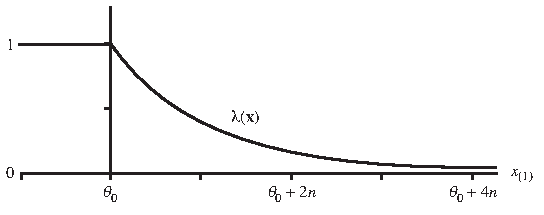
\includegraphics[width=.85\textwidth]{assets/chapter8/fig8-2-1.pdf}
\caption{$\lambda(\boldsymbol x)$，一个仅依赖于 $x_{(1)}$ 的函数.}\label{fig:8.2.1}
\end{figure}

\autoref{fig:8.2.1}画出了 $\lambda(\boldsymbol x)$. 似然比检验在 $\lambda(\boldsymbol X)\le c$ 时拒绝 $H_0$，其拒绝域是 $\{\boldsymbol x:x_{(1)}\ge\theta_0-(\log c)/n\}$.\footnote{译注：这一拒绝域的改写适用于 $0<c<1$. 若取定义允许的端点 $c=1$，由 $\lambda\le1$ 应拒绝全部样本，而所写集合仅含 $x_{(1)}\ge\theta_0$ 的样本；$c=0$ 时则无有限样本被拒绝，涉及 $\log0$ 的表达式应作极限理解.} 注意，拒绝域仅通过充分统计量 $X_{(1)}$ 依赖样本. \autoref{thm:8.2.4}将说明，这一现象普遍成立.
\end{example}
\autoref{ex:8.2.3}再次说明\autoref{sec:7.2.2}指出的一点：对似然函数求导，并不是求最大似然估计量的唯一方法. 在该例中，$L(\theta\mid\boldsymbol x)$ 在 $\theta=x_{(1)}$ 处不可微.

若 $T(\boldsymbol X)$ 是 $\theta$ 的充分统计量，密度或质量函数为 $g(t\mid\theta)$，则可以考虑用 $T$ 及其似然函数 $L^*(\theta\mid t)=g(t\mid\theta)$ 构造似然比检验，而不直接使用样本 $\boldsymbol X$ 及其似然函数 $L(\theta\mid\boldsymbol x)$. 用 $\lambda^*(t)$ 表示基于 $T$ 的似然比检验统计量. 直观上，$\boldsymbol x$ 中关于 $\theta$ 的全部信息都包含在 $T(\boldsymbol x)$ 中，因此基于 $T$ 的检验应当与基于完整样本的检验一样好. 事实上，这两种检验等价.
\begin{theorem}\label{thm:8.2.4}\index{SI0642@充分统计量}
若 $T(\boldsymbol X)$ 是 $\theta$ 的充分统计量，$\lambda^*(t)$ 和 $\lambda(\boldsymbol x)$ 分别为基于 $T$ 与 $\boldsymbol X$ 的似然比检验统计量，则对样本空间中的每个 $\boldsymbol x$，$\lambda^*(T(\boldsymbol x))=\lambda(\boldsymbol x)$.
\end{theorem}
\sourcepageanchor{337}
\begin{proof}
由因子分解定理（\autoref{thm:6.2.6}），$\boldsymbol X$ 的密度或质量函数可写为 $f(\boldsymbol x\mid\theta)=g(T(\boldsymbol x)\mid\theta)h(\boldsymbol x)$，其中 $g(t\mid\theta)$ 是 $T$ 的密度或质量函数，$h(\boldsymbol x)$ 不依赖于 $\theta$. 因此，
$$\begin{aligned}
\lambda(\boldsymbol x)&=\frac{\sup_{\Theta_0}L(\theta\mid\boldsymbol x)}{\sup_\Theta L(\theta\mid\boldsymbol x)}
=\frac{\sup_{\Theta_0}f(\boldsymbol x\mid\theta)}{\sup_\Theta f(\boldsymbol x\mid\theta)}\\
&=\frac{\sup_{\Theta_0}g(T(\boldsymbol x)\mid\theta)h(\boldsymbol x)}{\sup_\Theta g(T(\boldsymbol x)\mid\theta)h(\boldsymbol x)}&&\text{（$T$ 充分）}\\
&=\frac{\sup_{\Theta_0}g(T(\boldsymbol x)\mid\theta)}{\sup_\Theta g(T(\boldsymbol x)\mid\theta)}&&\text{（$h$ 不依赖于 $\theta$）}\\
&=\frac{\sup_{\Theta_0}L^*(\theta\mid T(\boldsymbol x))}{\sup_\Theta L^*(\theta\mid T(\boldsymbol x))}&&\text{（$g$ 是 $T$ 的密度或质量函数）}\\
&=\lambda^*(T(\boldsymbol x)).
\end{aligned}$$
\end{proof}
\autoref{ex:8.2.2}之后指出，求出 $\lambda(\boldsymbol x)$ 的表达式后，应设法将它化简. 根据\autoref{thm:8.2.4}，这句话的一种解释是：若 $T(\boldsymbol X)$ 是 $\theta$ 的充分统计量，则化简后的 $\lambda(\boldsymbol x)$ 应仅通过 $T(\boldsymbol x)$ 依赖于 $\boldsymbol x$.
\begin{example}[似然比检验与充分性]\label{ex:8.2.5}\index{SI0634@指数}
在\autoref{ex:8.2.2}中，可以看出 $\bar X$ 是 $\theta$ 的充分统计量. 利用 $\bar X$ 的似然函数（$\bar X\sim\mathrm n(\theta,1/n)$），可以更容易得到结论：检验 $H_0:\theta=\theta_0$ 对 $H_1:\theta\ne\theta_0$ 的似然比检验在 $|\bar X-\theta_0|$ 较大时拒绝 $H_0$.

类似地，在\autoref{ex:8.2.3}中，$X_{(1)}=\min X_i$ 是 $\theta$ 的充分统计量. $X_{(1)}$ 的似然函数（即其概率密度函数）为
$$L^*(\theta\mid x_{(1)})=\begin{cases}ne^{-n(x_{(1)}-\theta)},&\theta\le x_{(1)},\\0,&\theta>x_{(1)}.\end{cases}$$
也可利用这一似然函数，推出 $H_0:\theta\le\theta_0$ 对 $H_1:\theta>\theta_0$ 的似然比检验在 $X_{(1)}$ 较大时拒绝 $H_0$.
\end{example}
似然比检验对于存在干扰参数（nuisance parameters）\index{SI0727@滋扰参数}\semanticindexanchor{727:337}的情况也很有用；干扰参数是模型中存在、却不是推断直接关心的参数. 它们的存在不影响似然比检验的构造方法，但正如可能预料到的，它们可能导致不同的检验.
\begin{example}[方差未知时正态总体的似然比检验]\label{ex:8.2.6}\index{SI0638@正态}\index{SI0639@滋扰参数}\index{SI1019@似然比检验}
设 $X_1,\ldots,X_n$ 是来自 $\mathrm n(\mu,\sigma^2)$ 的随机样本，实验者只关心关于 $\mu$ 的推断，例如检验 $H_0:\mu\le\mu_0$ 对 $H_1:\mu>\mu_0$. 此时 $\sigma^2$ 是干扰参数. 似然比检验统计量为\footnote{译注：原文在最大化范围中写 $\sigma^2\ge0$，但所用普通正态密度要求 $\sigma^2>0$. $\sigma^2=0$ 对应退化分布，不能直接代入该密度；正文保留原范围.}
$$\begin{aligned}
\lambda(\boldsymbol x)&=\frac{\max_{\{\mu,\sigma^2:\mu\le\mu_0,\,\sigma^2\ge0\}}L(\mu,\sigma^2\mid\boldsymbol x)}{\max_{\{\mu,\sigma^2:-\infty<\mu<\infty,\,\sigma^2\ge0\}}L(\mu,\sigma^2\mid\boldsymbol x)}\\
&=\frac{\max_{\{\mu,\sigma^2:\mu\le\mu_0,\,\sigma^2\ge0\}}L(\mu,\sigma^2\mid\boldsymbol x)}{L(\hat\mu,\hat\sigma^2\mid\boldsymbol x)},
\end{aligned}$$
\sourcepageanchor{338}
其中 $\hat\mu$ 与 $\hat\sigma^2$ 是 $\mu$ 和 $\sigma^2$ 的最大似然估计量（\autoref{ex:7.2.11}\mbox{）.} 进一步，若 $\hat\mu\le\mu_0$，约束最大值与无约束最大值相同；若 $\hat\mu>\mu_0$，则约束最大值为 $L(\mu_0,\hat\sigma_0^2\mid\boldsymbol x)$，其中 $\hat\sigma_0^2=\sum(x_i-\mu_0)^2/n$. 因此，
$$\lambda(\boldsymbol x)=\begin{cases}1,&\hat\mu\le\mu_0,\\\dfrac{L(\mu_0,\hat\sigma_0^2\mid\boldsymbol x)}{L(\hat\mu,\hat\sigma^2\mid\boldsymbol x)},&\hat\mu>\mu_0.\end{cases}$$
经过一些代数运算，可以证明基于 $\lambda(\boldsymbol x)$ 的检验等价于基于 Student 的 $t$ 统计量的检验. 细节留作\autoref{exercise:8.37}. （\autoref{exercise:8.38}至\autoref{exercise:8.42}也讨论干扰参数问题.）
\end{example}

\subsubsection{贝叶斯检验}\label{sec:8.2.2}
假设检验问题也可以用贝叶斯模型表述. 回顾\autoref{sec:7.2.3}，贝叶斯模型不仅包含抽样分布 $f(\boldsymbol x\mid\theta)$，还包含先验分布 $\pi(\theta)$；先验分布反映实验者在抽样前对参数 $\theta$ 的看法.

贝叶斯范式要求用贝叶斯定理把样本信息与先验信息结合起来，得到后验分布 $\pi(\theta\mid\boldsymbol x)$. 此后关于 $\theta$ 的全部推断都以这个后验分布为依据.

在假设检验问题中，可以用后验分布计算 $H_0$ 与 $H_1$ 为真的概率. 要记住，$\pi(\theta\mid\boldsymbol x)$ 是一个随机变量的概率分布，因此可以计算后验概率
$$P(\theta\in\Theta_0\mid\boldsymbol x)=P(H_0\text{ 为真}\mid\boldsymbol x),\qquad
P(\theta\in\Theta_0^c\mid\boldsymbol x)=P(H_1\text{ 为真}\mid\boldsymbol x).$$
对经典统计学家而言，$P(H_0\text{ 为真}\mid\boldsymbol x)$ 和 $P(H_1\text{ 为真}\mid\boldsymbol x)$ 没有意义. 经典统计学家把 $\theta$ 看成固定的数，因此一个假设非真即假. 若 $\theta\in\Theta_0$，则对所有 $\boldsymbol x$，$P(H_0\text{ 为真}\mid\boldsymbol x)=1$，$P(H_1\text{ 为真}\mid\boldsymbol x)=0$. 若 $\theta\in\Theta_0^c$，这两个值就颠倒过来. 因为这些概率未知（$\theta$ 未知），且不依赖样本 $\boldsymbol x$，经典统计学家不使用它们. 在假设检验的贝叶斯表述中，这些概率依赖样本 $\boldsymbol x$，能提供有关 $H_0$ 和 $H_1$ 真伪的有用信息.

贝叶斯检验者使用后验分布的一种方式是：当 $P(\theta\in\Theta_0\mid\boldsymbol X)\ge P(\theta\in\Theta_0^c\mid\boldsymbol X)$ 时，接受 $H_0$ 为真，否则拒绝 $H_0$. 用前几节的术语来说，作为样本函数的检验统计量是 $P(\theta\in\Theta_0^c\mid\boldsymbol X)$，拒绝域是 $\{\boldsymbol x:P(\theta\in\Theta_0^c\mid\boldsymbol x)>1/2\}$. 另一种做法是：若希望防范错误拒绝 $H_0$，可以决定仅在 $P(\theta\in\Theta_0^c\mid\boldsymbol X)$ 超过某个很大的数（例如 $.99$）时才拒绝 $H_0$.
\begin{example}[正态总体的贝叶斯检验]\label{ex:8.2.7}\index{SI0488@正态}
设 $X_1,\ldots,X_n$ 独立同分布于 $\mathrm n(\theta,\sigma^2)$，$\theta$ 的先验分布为 $\mathrm n(\mu,\tau^2)$，其中 $\sigma^2,\mu,\tau^2$ 已知. 考虑检验 $H_0:\theta\le\theta_0$ 对 $H_1:\theta>\theta_0$. 由\autoref{ex:7.2.16}，后验分布 $\pi(\theta\mid\boldsymbol x)$ 为正态分布，均值为 $(n\tau^2\bar x+\sigma^2\mu)/(n\tau^2+\sigma^2)$，方差为 $\sigma^2\tau^2/(n\tau^2+\sigma^2)$.

若决定当且仅当 $P(\theta\in\Theta_0\mid\boldsymbol X)\ge P(\theta\in\Theta_0^c\mid\boldsymbol X)$ 时接受 $H_0$，则接受 $H_0$ 当且仅当
$$\frac12\le P(\theta\in\Theta_0\mid\boldsymbol X)=P(\theta\le\theta_0\mid\boldsymbol X).$$
由于 $\pi(\theta\mid\boldsymbol x)$ 对称，此式成立当且仅当后验均值不大于 $\theta_0$. 因此，若
$$\bar X\le\theta_0+\frac{\sigma^2(\theta_0-\mu)}{n\tau^2},$$
\sourcepageanchor{339}
则接受 $H_0$ 为真，否则接受 $H_1$ 为真. 特别地，若 $\mu=\theta_0$，即实验前赋予 $H_0$ 和 $H_1$ 的概率均为 $1/2$，那么当 $\bar x\le\theta_0$ 时接受 $H_0$ 为真，否则接受 $H_1$.
\end{example}
\autoref{sec:8.3.5}将讨论在假设检验问题中利用后验分布作推断的其他方法.

\subsubsection{并交检验与交并检验}\label{sec:8.2.3}
在某些情形下，可以从简单原假设的检验构造复杂原假设的检验. 我们讨论两种相关方法.

当原假设便于写成一个交集时，并交法（union–intersection method）可能很有用，例如
\begin{equation}\label{eq:8.2.3}H_0:\theta\in\bigcap_{\gamma\in\Gamma}\Theta_\gamma.\end{equation}
这里 $\Gamma$ 是任意指标集，依问题不同可以有限，也可以无限. 假设每个检验 $H_{0\gamma}:\theta\in\Theta_\gamma$ 对 $H_{1\gamma}:\theta\in\Theta_\gamma^c$ 的问题，都已有可用的检验. 设检验 $H_{0\gamma}$ 的拒绝域为 $\{\boldsymbol x:T_\gamma(\boldsymbol x)\in R_\gamma\}$. 则并交检验（union–intersection test）的拒绝域为
\begin{equation}\label{eq:8.2.4}\index{SI0522@并交}\bigcup_{\gamma\in\Gamma}\{\boldsymbol x:T_\gamma(\boldsymbol x)\in R_\gamma\}.\end{equation}
道理很简单：只要任一 $H_{0\gamma}$ 被拒绝，$H_0$ 也必须被拒绝，因为由\eqref{eq:8.2.3}，$H_0$ 为真仅当每个 $H_{0\gamma}$ 都为真. 只有每个 $H_{0\gamma}$ 都被接受为真，交集 $H_0$ 才会被接受为真.

有时，并交检验的拒绝域可以写得很简单. 特别地，假设每个单独检验的拒绝域都形如 $\{\boldsymbol x:T_\gamma(\boldsymbol x)>c\}$，其中 $c$ 不依赖于 $\gamma$. 则\eqref{eq:8.2.4}可写为
$$\bigcup_{\gamma\in\Gamma}\{\boldsymbol x:T_\gamma(\boldsymbol x)>c\}
=\{\boldsymbol x:\sup_{\gamma\in\Gamma}T_\gamma(\boldsymbol x)>c\}.$$
所以，检验 $H_0$ 的统计量是 $T(\boldsymbol x)=\sup_{\gamma\in\Gamma}T_\gamma(\boldsymbol x)$. \autoref{sec:11}给出了一些 $T(\boldsymbol x)$ 具有简单公式的例子.
\begin{example}[正态总体的并交检验]\label{ex:8.2.8}\index{SI0525@正态}\index{SI1021@双侧}
设 $X_1,\ldots,X_n$ 是来自 $\mathrm n(\mu,\sigma^2)$ 总体的随机样本. 考虑检验 $H_0:\mu=\mu_0$ 对 $H_1:\mu\ne\mu_0$，$\mu_0$ 为指定数. 可把 $H_0$ 写成两个集合的交：
$$H_0:\{\mu:\mu\le\mu_0\}\cap\{\mu:\mu\ge\mu_0\}.$$
检验 $H_{0L}:\mu\le\mu_0$ 对 $H_{1L}:\mu>\mu_0$ 的似然比检验为
$$\text{若 }\frac{\bar X-\mu_0}{S/\sqrt n}\ge t_L,\quad\text{则拒绝 $H_{0L}:\mu\le\mu_0$，支持 $H_{1L}:\mu>\mu_0$}$$
（见\autoref{exercise:8.37}\mbox{）.} 类似地，检验 $H_{0U}:\mu\ge\mu_0$ 对 $H_{1U}:\mu<\mu_0$ 的似然比检验为
$$\text{若 }\frac{\bar X-\mu_0}{S/\sqrt n}\le t_U,\quad\text{则拒绝 $H_{0U}:\mu\ge\mu_0$，支持 $H_{1U}:\mu<\mu_0$}.$$
由这两个似然比检验构成的并交检验，检验 $H_0:\mu=\mu_0$ 对 $H_1:\mu\ne\mu_0$，其规则为
$$\text{若 }\frac{\bar X-\mu_0}{S/\sqrt n}\ge t_L\quad\text{或}\quad\frac{\bar X-\mu_0}{S/\sqrt n}\le t_U,\quad\text{则拒绝 }H_0.$$
\sourcepageanchor{340}
若 $t_L=-t_U\ge0$，则可更简洁地写为
$$\text{若 }\frac{|\bar X-\mu_0|}{S/\sqrt n}\ge t_L,\quad\text{则拒绝 }H_0.$$
事实上，这个并交检验也是该问题的似然比检验（见\autoref{exercise:8.38}），称为双侧 $t$ 检验（two-sided $t$ test\mbox{）.}
\end{example}
原假设便于写成交集时，并交构造法很有用. 另一种方法——交并法（intersection–union method）——则可能适用于原假设便于写成并集的情形. 假设要检验的原假设为
\begin{equation}\label{eq:8.2.5}H_0:\theta\in\bigcup_{\gamma\in\Gamma}\Theta_\gamma.\end{equation}
假设对每个 $\gamma\in\Gamma$，$\{\boldsymbol x:T_\gamma(\boldsymbol x)\in R_\gamma\}$ 是检验 $H_{0\gamma}:\theta\in\Theta_\gamma$ 对 $H_{1\gamma}:\theta\in\Theta_\gamma^c$ 的拒绝域. 则检验 $H_0$ 对 $H_1$ 的交并检验（intersection–union test）的拒绝域为
\begin{equation}\label{eq:8.2.6}\index{SI0494@交并}\bigcap_{\gamma\in\Gamma}\{\boldsymbol x:T_\gamma(\boldsymbol x)\in R_\gamma\}.\end{equation}
由\eqref{eq:8.2.5}，$H_0$ 为假当且仅当所有 $H_{0\gamma}$ 都为假，所以仅当每个单独假设 $H_{0\gamma}$ 都可拒绝时，$H_0$ 才可拒绝. 同样，若单独假设的拒绝域都形如 $\{\boldsymbol x:T_\gamma(\boldsymbol x)\ge c\}$（$c$ 与 $\gamma$ 无关），检验就可大为简化. 此时 $H_0$ 的拒绝域为
$$\bigcap_{\gamma\in\Gamma}\{\boldsymbol x:T_\gamma(\boldsymbol x)\ge c\}
=\{\boldsymbol x:\inf_{\gamma\in\Gamma}T_\gamma(\boldsymbol x)\ge c\}.$$
交并检验在检验统计量 $\inf_{\gamma\in\Gamma}T_\gamma(\boldsymbol X)$ 较大时拒绝 $H_0$.
\begin{example}[验收抽样]\label{ex:8.2.9}\index{SI0002@验收抽样}\index{SI0495@伯努利}\index{SI0497@正态}
本例说明，验收抽样是交并检验一个极有用的应用领域. （关于这个问题更详细的讨论，见 \hyperref[bib:source23]{Berger (1982)}.）

评估家具装饰织物质量时，两个重要参数是平均断裂强度 $\theta_1$ 和通过燃烧性能试验的概率 $\theta_2$. 标准可能规定 $\theta_1$ 应超过 $50$ 磅，$\theta_2$ 应超过 $.95$；只有两项均达标，织物才可接受. 可以用下列假设检验建模：
$$H_0:\{\theta_1\le50\text{ 或 }\theta_2\le.95\}\quad\text{对}\quad
H_1:\{\theta_1>50\text{ 且 }\theta_2>.95\},$$
只有接受 $H_1$，这批材料才予以验收.

假设 $X_1,\ldots,X_n$ 是 $n$ 个样品的断裂强度测量值，并假定它们独立同分布于 $\mathrm n(\theta_1,\sigma^2)$. $H_{01}:\theta_1\le50$ 的似然比检验，在 $(\bar X-50)/(S/\sqrt n)>t$ 时拒绝 $H_{01}$. 又假设还获得了 $m$ 次燃烧性能试验的结果 $Y_1,\ldots,Y_m$；第 $i$ 个样品通过试验时 $Y_i=1$，否则 $Y_i=0$. 若将它们建模为独立同分布的 $\operatorname{Bernoulli}(\theta_2)$ 随机变量，则似然比检验在 $\sum_{i=1}^mY_i>b$ 时拒绝 $H_{02}:\theta_2\le.95$（见\autoref{exercise:8.3}\mbox{）.} 合起来，交并检验的拒绝域为
$$\left\{(\boldsymbol x,\boldsymbol y):\frac{\bar x-50}{s/\sqrt n}>t\text{ 且 }\sum_{i=1}^my_i>b\right\}.$$
因此，这个交并检验判定产品可接受、即 $H_1$ 为真，当且仅当它判定每个单独参数都符合相应标准、即 $H_{1i}$ 为真. 若产品质量由两个以上参数定义，可以用交并法组合各参数的单独检验，得到产品质量的总体检验.
\end{example}
